\documentclass[11pt,a4paper]{article}

\usepackage[margin=1in]{geometry}
\usepackage{graphicx}
\usepackage{hyperref}
\usepackage{amsmath,amssymb}
\usepackage{mathtools}

\title{High-Level Structure of Dependency Networks}

\author{Alexei Vazquez\\
\small Nodes \& Links Ltd, Salisbury House, Station Road, Cambridge, CB1 2LA, UK\\
\small \texttt{alexei@nodeslinks.com}}

\date{}

\begin{document}

\maketitle

\begin{abstract}
Dependency networks describe how activities, events or processes are linked by prerequisite relationships, but real networks are often too large to interpret directly. Here we ask how to summarise such a network at a higher level of organisation, using construction project schedules as a case study. We introduce two simple, deterministic ways of grouping activities: the Dependency Uprise Structure (DUS), which collects activities that share the same logical depth in the network, and the Dependency Fibration Structure (DFS), which refines this grouping by also recording which earlier levels each activity depends on. Applied to construction projects, the DUS compresses the original dependency network exponentially and the DFS provides an intermediate, sub-linear summary. Both reveal a small-world organisation that is hidden in the raw schedule. Because dependency networks appear in fields as diverse as project management, causal inference, ancestry analysis and neural networks, the same approach should generalise well beyond construction. A Python implementation is available at \url{https://github.com/av2atgh/dus}.
\end{abstract}

\section*{Introduction}

Most large human endeavours are organised as projects \cite{jensen16, schoper2017projectification, wagner2021projectification}. A building is constructed, a piece of software is delivered, or a new drug is brought through clinical trials by coordinating many smaller activities under shared deadlines and budgets. Although the products are very different, the underlying logistics are remarkably similar, and the discipline of project management has emerged to plan and control them across sectors.

Coordinating a project of any size requires a high-level framework that connects day-to-day execution with strategic goals \cite{pmi2021pmbok, taxen2011system}. Almost universally, this is achieved by breaking the total work into smaller, manageable units that can be assigned to teams, costed, scheduled and tracked. The way the work is broken down determines how progress is monitored and how risks are spotted.

The standard tool for this decomposition is the Work Breakdown Structure (WBS) \cite{pmi2021pmbok}. The WBS is a tree of deliverables: the final product sits at the top and is recursively divided into ever smaller pieces of work, until the leaves are activities small enough to be scheduled and budgeted individually. The resulting hierarchy is the backbone of project planning, organising responsibilities and providing a common map for everyone involved.

The WBS captures what needs to be done, but not the order in which it has to happen. To turn a list of activities into a schedule, the project manager must specify which activities are prerequisites for which others --- the foundation of a building must be poured before the frame goes up, or a back-end service must be available before its front-end can be tested. The set of these prerequisite relationships forms a {\em dependency network}. From this network one can compute the critical path, identify slack, and estimate when the project will end.

Project teams therefore look at their work through two different lenses: the deliverable-based hierarchy of the WBS and the prerequisite-based wiring of the dependency network. These two views rarely line up, because dependencies routinely cross WBS boundaries. What is missing is a high-level summary of the dependency network itself --- not a top-down decomposition imposed from above, but a structure that emerges from the dependencies. Recovering such a summary is an inverse problem: instead of starting with a goal and dividing it, we start with the fine-grained dependencies and try to expose their large-scale organisation.

Network science has long studied related inverse problems, developing increasingly sophisticated statistical methods to find communities and other meso-scale structure in graphs \cite{radicchi_communities_2004, newman_communities_2006, hofman_communities_2008, karrer_blockmodels_2011, peixoto2025}. These methods have rarely been applied to dependency networks. As we show below, the dependency case is in fact considerably simpler: a useful high-level structure can be extracted deterministically, without statistical inference, by exploiting the directional, acyclic nature of the network.

\section*{Results}

\subsection*{Dependency Uprise Structure}

In a dependency network each node is an activity and each directed link encodes a prerequisite, with $A \to B$ meaning that activity $A$ must finish before activity $B$ can start. Such networks are directed graphs \cite{gross2005graph}. They must also be acyclic: a loop such as $A \to B \to C \to A$ would require $A$ to be finished before it can begin. Dependency networks are therefore directed acyclic graphs (DAGs) \cite{gross2005graph}.

Every DAG admits a {\em topological order}: an arrangement of its nodes in which all of an activity's predecessors come before it and all of its successors come after it. Some orderings are forced, as in the chain $A_{1} \to A_{2} \to A_{3} \to \dots \to A_{n}$, while others leave room for choice. If $A_{1}$ feeds both $A_{2}$ and $A'_{2}$ and both must finish before $A_{3}$ starts, then $A_{2}$ and $A'_{2}$ can be swapped without changing anything that matters for the schedule. This freedom motivates assigning every activity an integer that measures how many dependency steps separate it from a starting activity, made precise below.

We assign DUS index $u_i = 0$ to every activity with no predecessors, and otherwise
%
\begin{equation}
u_i = 1 + \max_{j\in \text{PredecessorsOf}(i)} u_j.
\label{DUS_definition}
\end{equation}
%
After processing all activities in a topological order, $u_i$ equals the length of the longest dependency chain leading to activity $i$. The Dependency Uprise Structure (DUS) is the partition of activities by this index: each DUS subset contains the activities sharing one value of $u_i$. By construction, two activities sharing a DUS index are pairwise incomparable in the dependency DAG --- neither is a predecessor of the other --- so they can appear in either relative order within a valid topological sort. The converse does not hold: two activities at different depths can also be incomparable, so the DUS is one specific antichain decomposition of the DAG, not in general the coarsest one.

The construction in (\ref{DUS_definition}) is analogous to the layering used in the first phase of the Sugiyama framework for hierarchical graph drawing \cite{sugiyama1981} and is closely related to the Coffman--Graham scheduling algorithm \cite{coffmangraham1972}. The novel contribution of this paper is not the layering itself but its use as a coarse-graining of the dependency network, the empirical scaling laws established below for construction project schedules, and the finer DFS construction introduced in the section on the DUS fine structure.

\subsection*{The DUS network}

Once activities have been grouped into DUS levels, we can collapse the original dependency network onto these groups. In the resulting DUS network each node is a DUS, and a weighted edge $U_a \xrightarrow{w_{ab}} U_b$ records that $w_{ab}$ activity-level dependencies run from members of $U_a$ to members of $U_b$. The DUS network inherits the directed acyclic structure of the dependency network. What is new is the weight $w_{ab}$, which measures how strongly two DUS levels are coupled.

The simplest DUS network is a chain, for example $U_0 \xrightarrow{w_{01}} U_1 \xrightarrow{w_{12}} U_2$. In general, dependencies may also skip ahead, linking distant levels. A chain through every level is, however, always present: by the definition of $u_i$ in (\ref{DUS_definition}), every activity has at least one predecessor in the previous DUS, so $w_{i-1,\,i} \geq 1$. The chain $U_0 \to U_1 \to U_2 \to \cdots \to U_{m-1}$, where $m$ is the number of DUSs, is therefore the longest path in the DUS network. We call it the {\em DUS spine}, by analogy to the activity-level critical path while avoiding overlap with that term's specific duration-weighted meaning in project management.

\begin{figure}[t]
\centering
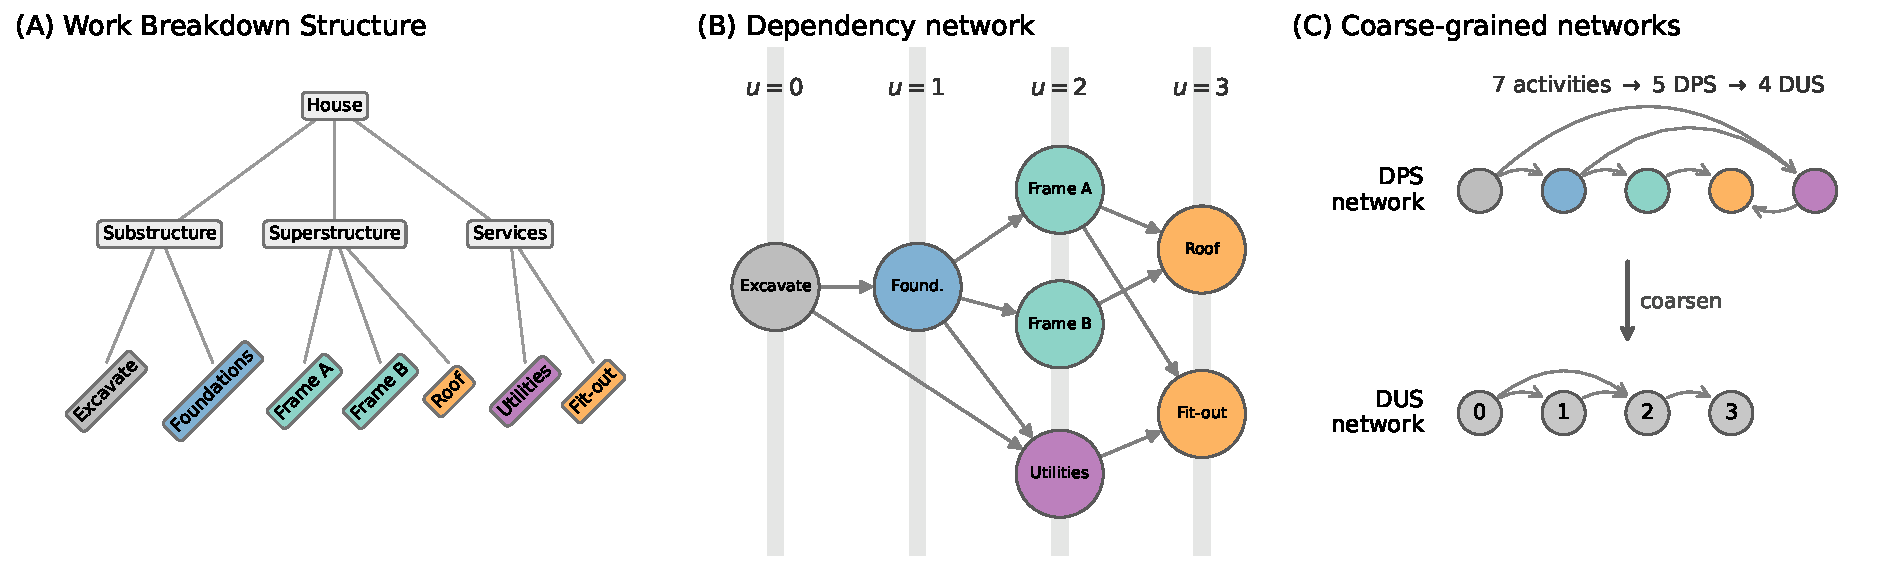
\includegraphics[width=0.85\linewidth]{fig1.pdf}
\caption{DUS networks. (A,B) DUS networks of two construction project schedules. The nodes represent DUSs, ordered from left to right according to their position along the DUS spine. The links represent dependencies between DUSs, with the grey scale proportional to their number. (C, D) Adding the number of activities in each DUS (bar heights) and current progress (colour map).}
\label{examples}
\end{figure}

Figure \ref{examples}A, B shows the DUS networks of two construction project schedules drawn from the Nodes \& Links database (see Methods). Each DUS appears as a dot, arranged from left to right along the DUS spine; arcs above the spine represent extra dependencies between non-adjacent DUSs, with darker arcs encoding more dependencies. Because the DUS network is small enough to draw, it offers a natural canvas on which to overlay other project information. In Figure \ref{examples}C, D the height of each bar is proportional to the number of activities in the corresponding DUS, and the colour encodes the Physical Progress Percent, a standard progress metric in construction. We refer to this composite display as the {\em DUS profile}.

\subsection*{Scaling properties}

\begin{figure}[t]
\centering
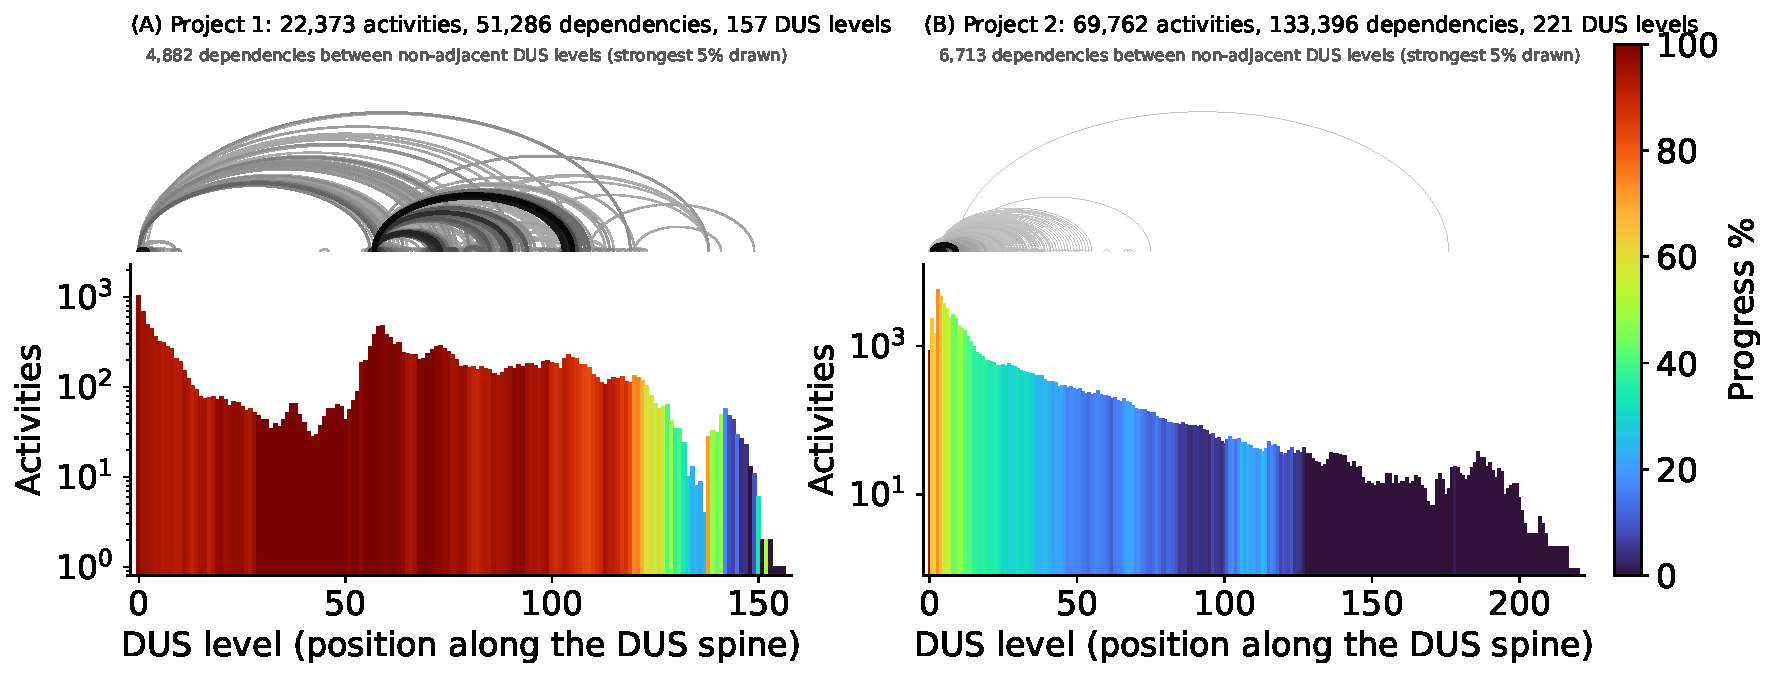
\includegraphics[width=0.7\linewidth]{fig2.pdf}
\caption{Scaling of the number of DUSs and the number of dependencies. Each point represents a construction project. The dashed line is a fit to the scaling law $y = p \log(x)$ using all data points. Colours correspond to projects from three different construction companies.}
\label{scaling_size}
\end{figure}

\begin{figure}[t]
\centering
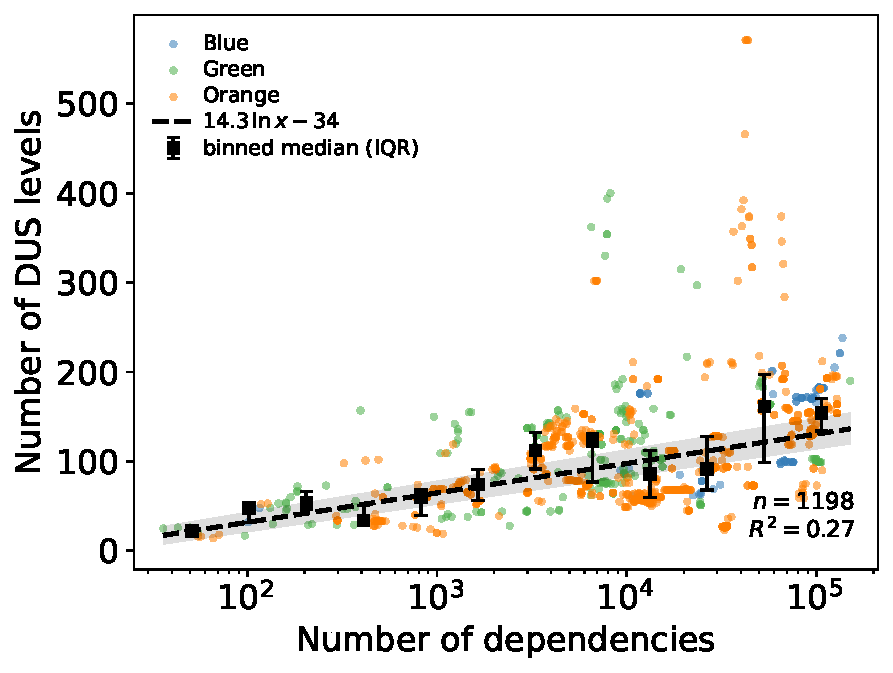
\includegraphics[width=0.7\linewidth]{fig3.pdf}
\caption{DUS networks are small worlds. Average distance between every DUS and the ending DUS versus the number of DUSs in the project schedule. Each point represents a construction project. Colours correspond to projects from three different construction companies.}
\label{scaling_distance}
\end{figure}

To probe how the DUS network scales with project size we collected schedules from three construction companies, identified below as blue, green and orange (see Methods). The number of DUSs grows only logarithmically with the number of activity-level dependencies (Figure \ref{scaling_size}), and the same relation describes all three companies. The DUS network is therefore an exponential compression of the underlying dependency network: doubling the size of the project adds only a constant number of DUS levels.

A second question is how far apart, on average, two DUSs are in the network. If a project had no dependencies outside the DUS spine, the mean distance from any DUS to the final one would be exactly $(m -1) / 2$. Real projects fall well below this expectation (points vs dashed line in Figure \ref{scaling_distance}): large DUS networks are much more tightly connected than their spines would suggest. The reason is that many dependencies act as shortcuts, linking DUSs that are far apart along the spine (see Figure \ref{examples}A, B). In this sense, the DUS networks of construction projects are small-worlds \cite{watts98}.

\subsection*{DUS fine structure}

\begin{figure}[t]
\centering
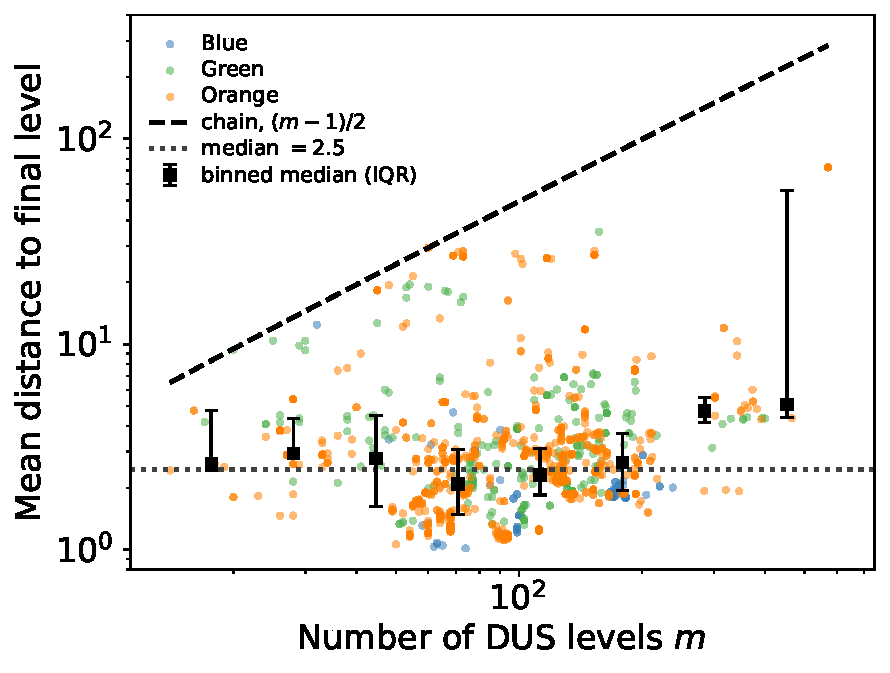
\includegraphics[width=0.7\linewidth]{fig4.pdf}
\caption{Nodes in a dependency network are stratified based on their dependency patterns. Node colour indicates the DFS, and the node label gives the DUS.}
\label{example}
\end{figure}

\begin{figure}[t]
\centering
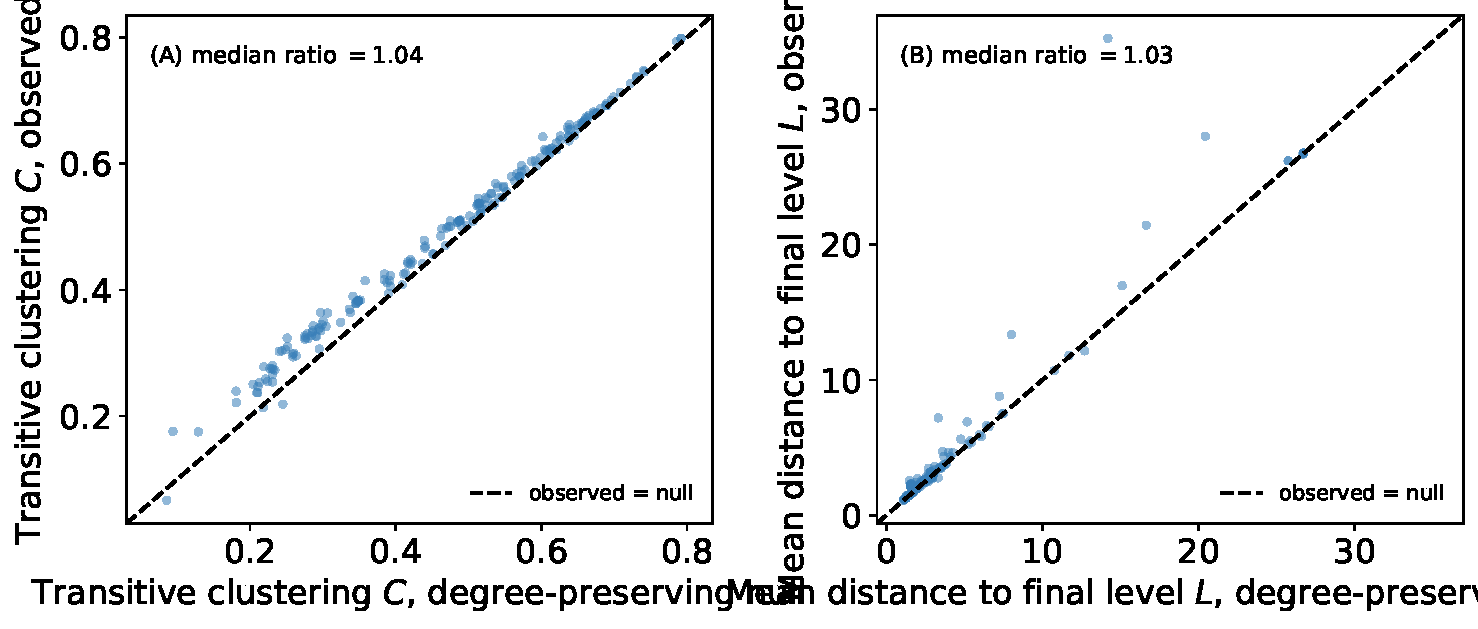
\includegraphics[width=0.7\linewidth]{fig5.pdf}
\caption{Scaling of the number of DFSs and the number of dependencies. Each point represents a construction project. The dashed line is a fit to the scaling law $y = p x^{q}$ using all data points. Colours correspond to projects from three different construction companies.}
\label{scaling_dfs}
\end{figure}

Activities sharing the same DUS index can be further split according to the DUS levels their predecessors come from (Figure \ref{example}). An activity at $DUS = i$ must have at least one predecessor at $DUS = i-1$; predecessors at $DUS = 0, \ldots, i-2$ are optional. Each of the $i-1$ optional levels can be either present or absent, giving $2^{i-1}$ distinguishable predecessor patterns at the $i$-th DUS. (Activities at $DUS = 0$ have no predecessors, and those at $DUS = 1$ draw exclusively from $DUS = 0$, so neither can be split further.)

These finer groupings are related to what mathematicians call {\em graph fibrations} \cite{boldi2002fibration, morone2020fibrations}; we refer to them as the {\em Dependency Fibration Structure} (DFS) of the network. Restricting to DAGs again simplifies things, because each DFS can be labelled by a single integer. We set $f_i = 0$ when $u_i = 0$ and otherwise
%
\begin{equation}
f_i= \sum_{k=0}^{u_i - 2} b_{ik}\, 2^{k} + 2^{u_i - 1}
\label{dfs_definition}
\end{equation}
%
where $b_{ik}=1$ if activity $i$ has at least one predecessor in the $k$-th DUS and $b_{ik}=0$ otherwise. The integer $f_i$ should be read as a categorical label, not a metric: numerical proximity of two $f_i$ values does not imply similarity of their predecessor patterns.

As before, we collapse the dependency network onto its DFSs to obtain the DFS network: each node is a DFS, and a weighted edge $F_a \xrightarrow{w_{ab}} F_b$ records the $w_{ab}$ activity-level dependencies between them. Figure \ref{scaling_dfs} plots the number of DFSs in each project against the number of activity-level dependencies. The relation is sub-linear and well described by a power law (dashed line). The bound $2^{i-1}$ on patterns at level $i$ is therefore loose in practice: the realised count of distinct DFSs grows much more slowly than the worst case, and most theoretically possible patterns do not occur in real schedules. The DFS network sits between the original dependency network and the much smaller DUS network in terms of size.

\section*{Discussion}

Dependency networks admit two natural higher-level representations forming a chain of progressively coarser views, $\textit{Activity} \to \textit{DFS} \to \textit{DUS}$. For construction project schedules, the DFS provides a sub-linear coarse-graining and the DUS an exponential coarse-graining of the underlying dependency network. Both can be used directly for tracking and reporting, and both can serve as inputs to risk models that estimate project duration and cost.

Because the construction is purely topological, the same machinery applies to any system that can be represented as a directed acyclic graph, including causal networks, ancestries and feedforward neural networks. Two questions naturally follow. First, do the size scaling laws observed for construction schedules carry over to these other settings? Second, what features of the underlying dependency network determine the structure of its DFS and DUS networks, including the scaling between them?

\section*{Methods}

\subsection*{Dataset}

The construction project schedules analysed here were drawn from the Nodes \& Links database. Three construction companies are represented, identified throughout as blue, green and orange. Each company contributed several projects, allowing variation to be assessed both within a single organisation and across organisations. Activity-level dependencies and Physical Progress Percent values were taken directly from the schedules as recorded in the database.

\subsection*{Computation of the DUS and DFS}

The DUS index $u_i$ defined in equation (\ref{DUS_definition}) is computed by first sorting the activities into a topological order, then sweeping through that order and applying (\ref{DUS_definition}) to each activity in turn. The cost is linear in the number of activities plus the number of dependencies. The DFS index $f_i$ defined in equation (\ref{dfs_definition}) requires a single additional pass over the dependencies once $u_i$ is known: for each activity $i$ we record which lower DUS levels its predecessors occupy, and combine these bits into the integer label given by (\ref{dfs_definition}). The DUS and DFS networks are then obtained by collapsing the dependency network onto these labels and accumulating edge weights.

\subsection*{Code availability}

A Python implementation of the DUS and DFS algorithms, together with helper code to draw fish-plots, is available at \url{https://github.com/av2atgh/dus}.

\section*{Acknowledgements}

This research did not receive any specific grant from funding agencies in the public, commercial, or not-for-profit sectors. Nodes \& Links Ltd provided support in the form of salary for Alexei Vazquez but did not have any additional role in the conceptualisation of the study, the analysis, the decision to publish or the preparation of the manuscript.

\section*{Author contributions}

A.V. conceived the study, designed and implemented the algorithms, performed the analysis, prepared the figures and wrote the manuscript.

\section*{Use of generative AI}

The author used Claude (Anthropic) for language editing of the manuscript text. The tool was not used for the conception of the study, the design of the algorithms, the analysis of the data, the generation of figures, or the interpretation of results. All scientific content, claims and conclusions are the responsibility of the author.

%\bibliographystyle{unsrt}
%\bibliography{risk}

\begin{thebibliography}{10}

\bibitem{jensen16}
Anders Jensen, Christian Thuesen, and Joana Geraldi.
\newblock The {Projectification} of {Everything}: {Projects} as a {Human}
  {Condition}.
\newblock {\em Proj. Manag. J.}, 47(3):21--34, 2016.

\bibitem{schoper2017projectification}
Yvonne-Gabriele Schoper, Andreas Wald, Helgi~Thor Ingason, and Thordur~Vikingur
  Fridgeirsson.
\newblock Projectification in western economies: A comparative study of
  germany, norway and iceland.
\newblock {\em International Journal of Project Management}, 36(1):71--82,
  2018.
\newblock Festschrift for Professor J. Rodney Turner.

\bibitem{wagner2021projectification}
Reinhard Wagner, Martina Huemann, and Mladen Radujkovic.
\newblock The influence of project management associations on projectification
  of society – an institutional perspective.
\newblock {\em Project Leadership and Society}, 2:100021, 2021.

\bibitem{pmi2021pmbok}
{Project Management Institute}.
\newblock {\em A Guide to the Project Management Body of Knowledge
  (PMBOK{\textregistered} Guide)}.
\newblock Project Management Institute, Newtown Square, PA, seventh edition,
  2021.

\bibitem{taxen2011system}
Lars Tax{\'e}n.
\newblock {\em The System Anatomy – Enabling Agile Project Management}.
\newblock Studentlitteratur, Lund, 2011.

\bibitem{radicchi_communities_2004}
Filippo Radicchi, Claudio Castellano, Federico Cecconi, Vittorio Loreto, and
  Domenico Parisi.
\newblock Defining and identifying communities in networks.
\newblock {\em Proceedings of the National Academy of Sciences},
  101(9):2658--2663, 2004.

\bibitem{newman_communities_2006}
M.~E.~J. Newman.
\newblock Modularity and community structure in networks.
\newblock {\em Proceedings of the National Academy of Sciences},
  103(23):8577--8582, 2006.

\bibitem{hofman_communities_2008}
Jake~M. Hofman and Chris~H. Wiggins.
\newblock Bayesian approach to network modularity.
\newblock {\em Phys. Rev. Lett.}, 100:258701, Jun 2008.

\bibitem{karrer_blockmodels_2011}
Brian Karrer and M.~E.~J. Newman.
\newblock Stochastic blockmodels and community structure in networks.
\newblock {\em Phys. Rev. E}, 83:016107, Jan 2011.

\bibitem{peixoto2025}
Tiago~P. Peixoto.
\newblock Network reconstruction via the minimum description length principle.
\newblock {\em Phys. Rev. X}, 15:011065, Mar 2025.

\bibitem{gross2005graph}
Jonathan~L Gross and Jay Yellen.
\newblock {\em Graph Theory and Its Applications}.
\newblock Chapman and Hall/CRC, Boca Raton, FL, 2nd edition, 2005.

\bibitem{sugiyama1981}
Kozo Sugiyama, Shojiro Tagawa, and Mitsuhiko Toda.
\newblock Methods for visual understanding of hierarchical system structures.
\newblock {\em IEEE Transactions on Systems, Man, and Cybernetics},
  11(2):109--125, 1981.

\bibitem{coffmangraham1972}
E.~G. Coffman and R.~L. Graham.
\newblock Optimal scheduling for two-processor systems.
\newblock {\em Acta Informatica}, 1(3):200--213, 1972.

\bibitem{watts98}
Duncan~J. Watts and Steven~H. Strogatz.
\newblock Collective dynamics of ‘small-world’ networks.
\newblock {\em Nature}, 393(6684):440--442, June 1998.

\bibitem{boldi2002fibration}
Paolo Boldi and Sebastiano Vigna.
\newblock Fibrations of graphs.
\newblock {\em Discrete Mathematics}, 243(1):21--66, 2002.

\bibitem{morone2020fibrations}
Flaviano Morone, Ian Leifer, and Hernán~A. Makse.
\newblock Fibration symmetries uncover the building blocks of biological
  networks.
\newblock {\em Proceedings of the National Academy of Sciences},
  117(15):8306--8314, 2020.

\end{thebibliography}


\end{document}
